\chapter[Generalization Bounds with Complexity Measures]{\vspace{-0.7cm}Generalization Bounds with Complexity Measures}
\label{chap:dis-mu}
\addchapterlof
\addchapterloa
\addchapterloe

\vspace{-1.6cm}
\begin{center}
\textbf{This chapter is based on the following paper}\\
\end{center}
\vspace{-0.3cm}
\printpublication{ViallardEmonetHabrardMorvantZantedeschi2022}

\vspace{-0.3cm}
\minitoc

\vspace{-0.2cm}

\begin{abstract}
\vspace{-0.35cm}
{\small In statistical learning theory, generalization bounds usually involve a complexity measure that is constrained by the considered theoretical framework limiting the scope of such analysis.
Among the measured mentioned in this thesis (\Cref{chap:intro}) we can cite for example the VC-dimension, the stability constant of the uniform stability framework or the KL divergence used in the PAC-Bayesian framework studied in \Cref{part:contrib-pac-bayes}.
Recently, the empirical study of~\citet{JiangNeyshaburMobahiKrishnanBengio2020}, made in the context of neural networks learning, has shown that {\it (i)}~common complexity measures (such as the VC-dimension) do not necessarily correlate with the generalization gap, and that {\it (ii)}~there exist \textit{arbitrary} complexity measures that are better correlated with the generalization gap, but come without generalization guarantees.
In this chapter, we propose to address the second point by presenting a general framework allowing one to derive some generalization bounds able to take into account a general complexity measures.}
\end{abstract}

\newpage

\section{Introduction}

\looseness=-1
As shown in \Cref{chap:intro} and notably in \Cref{chap:intro:sec:bound}, statistical learning theory offers various theoretical frameworks to assess generalization by studying whether the empirical risk is representative of the true risk thanks to an upper bounding strategy of the generalization gap.
While the generalization gap represents a deviation between the true risk and the empirical risk, an upper bound on this generalization gap is generally a function of mainly two quantities: {\it (i)} the size of the training sample and {\it (ii)} a complexity measure that captures how much the model overfits the data.
There are some well-known complexity measures in the literature such as the VC-Dimension (\Cref{chap:intro:def:vc-dim}) or the Rademacher complexity (\Cref{chap:intro:def:rademacher}) that quantify how much a hypothesis from the hypothesis set can overfit the data. 
Following a different framework, instead of considering the whole hypothesis set, algorithmic-dependent complexity measures propose to quantify how much the hypothesis obtained by a learning algorithm overfit the data: the uniform stability (\Cref{chap:intro:def:stability}) or the robustness (\Cref{chap:intro:def:robustness}) parameters are two examples.\\

In order to study generalization capabilities, a recent line of works, mainly in the context of neural networks learning, is dedicated to the empirical study of different complexity measures to find those that correlate the most with the generalization gap~\citep{JiangNeyshaburMobahiKrishnanBengio2020,DziugaiteDrouinNealRajkumarCaballeroWangMitliagkasRoy2020,JiangNatekarSharma2021}. 
For example, given an arbitrary complexity measure, \citeauthor{JiangNeyshaburMobahiKrishnanBengio2020} estimate empirically the generalization gap and the complexity measure for over-parametrized models.
They are able to rank the measure and the gap to obtain the Kendall's rank coefficient~\citep{Kendall1938} to evaluate how a measure reflects the generalization for a particular model.
However, this correlation coefficient were criticized by~\citet{DziugaiteDrouinNealRajkumarCaballeroWangMitliagkasRoy2020} because they found that if the measures empirically correlate well {\it on average}, they are not robust to changes of the fixed parameters (such as the depth or the width of the model).\\

On the one hand, while these results are extremely important to understand generalization, notably for over-parametrized models, they remain incomplete since they are only empirical.
On the other hand, as we can see in \Cref{chap:intro:sec:bound}, the bounds in the literature are restrictive because the practitioner cannot integrate in a bound its own complexity measure.
In other words, to the best our knowledge, there is no generalization bound involving arbitrary complexity measures that are found to be good proxies for the generalization gap.
In this chapter, we aim to provide generalization bounds with arbitrary complexity measures that the practitioner can define.
We believe that this direction is of important interest in advancing the understanding of generalization, as the generalization gap can be {\it provably} upper-bounded with a term that depends on a user-specified complexity measure.
To get such generalization bounds, we leverage a disintegrated PAC-Bayesian bound (\Cref{chap:pac-bayes:theorem:general-disintegrated-rivasplata}).
Such a bound further allows to derive theoretical guarantees for arbitrary complexity measures that depend on the sampled model, and on the learning sample, which is uncommon in statistical learning theory.
Hence, our novel results provide theoretical foundation to the many regularization used in practice to perform model selection (\eg, L2 regularization).\\

The rest of the chapter is organized as follows. 
In \Cref{chap:dis-mu:sec:setting}, we provide some preliminaries dedicated to this chapter.
Then, we present the main contribution in \Cref{chap:dis-mu:sec:contrib,chap:dis-mu:sec:comparison} before concluding in \Cref{chap:dis-mu:sec:conclu}.
As usual in this thesis, in order to improve the readability of the chapter, the proofs are deferred in \Cref{ap:dis-mu}.

\section{Preliminaries}
\label{chap:dis-mu:sec:setting}

\looseness=-1
We provide in this section some quick recaps on notions that have been introduced previously in this thesis to make the reading easier. 
We first remind some elements about supervised learning and the generalization gap.
Then, we review quickly the disintegrated generalization bounds from which the contribution of this chapter are developed.

\subsection{Setting}
\label{chap:dis-mu:sec:notations}

We follow the setting of \Cref{chap:pac-bayes} and \Cref{chap:pac-bayes:sec:disintegrated} where we consider the supervised classification setting.
We recall that $\X$ denotes the input space and $\Y$ the label space.
Moreover, we consider that an example $(\x, \y)\in \X{\times}\Y$ is sampled from an unknown data distribution~$\D$ on $\X\times\Y$.
A learning sample $\S{=}\{(\x_i, \y_i)\}_{i=1}^\m$ contains $\m$ examples drawn \iid from $\D$; we denote the distribution of such an $\m$-sample by $\D^\m$.
Let $\H$ be a potentially infinite set of hypotheses $\h:\X{\to}\Y$ that associate a label belonging to $\Y$ given an input from $\X$.\\

Given a learning sample $\S$, we aim to find $\h \!\in\! \H$ that minimizes the so-called true risk $\Risk_{\D}(\h) {=} \PP_{(\x,\y)\sim\D}\LB h(x)\ne y\RB$.
In practice, as the data distribution $\D$ is unknown, we estimate the true risk with its empirical counterpart, \ie, the empirical risk $\Risk_{\dS}(\h) = \frac{1}{m}\sum_{i=1}^{m}\!\indic\LB h(x_i)\ne y_i\RB$.
We hereafter denote the generalization gap by $\phi: [0,1]^2\to\Rbb$, which is usually defined by $\phi(\Risk_{\D}(\h), \Risk_{\dS}(\h))=\vert\Risk_{\D}(\h){-}\Risk_{\dS}(\h)\vert$ that quantify how much the empirical risk is representative of the true risk.
Since the generalization bound is not computable, a complexity measure can be used to capture the overfitting phenomenon.\\

\looseness=-1
To incorporate arbitrary complexities in the bounds, we leverage the disintegrated PAC-Bayesian bounds framework (recalled in \Cref{chap:pac-bayes:sec:disintegrated}), \ie, we upper-bound the generalization gap for a hypothesis $\h$ sampled from $\AQ\in\M(\H)$ with a function that depends on an \textit{arbitrary} measure of complexity.
To do so, we need to consider an \apriori belief on the hypotheses in $\H$ that is modeled by a prior distribution $\P \in \M^{*}(\H)$.
Hence, we aim to learn, from $\S$ and $\P$, a {\it posterior} distribution $\AQ$ to assign higher probability to the best hypotheses in $\H$; the hypothesis $\h$ is then sampled from $\AQ$ to obtain the guarantee with an arbitrary complexity measure. 

\subsection{Reminder on Disintegrated PAC-Bayesian Bounds}
\label{chap:dis-mu:sec:disintegrated}

The disintegrated PAC-Bayesian bound (recalled in \Cref{chap:pac-bayes:sec:disintegrated}) has been introduced by \citet[Th~1.2.7]{Catoni2007} and \citet[Prop~3.1]{BlanchardFleuret2007}.
To the best of our knowledge, despite their interest, they have been little used in the literature and have only recently received renewed interest for deriving tight bounds in practice (see \Cref{chap:dis-pra}).
Such bounds take the following form (introduced in \Cref{chap:pac-bayes}).

\definitiondesintegrated*

Put into words, given a training set $\S$ sampled from $\D^\m$, we can learn the distribution $\AQ$ from $\S$, and then sample the hypothesis $\h$ from $\AQ$ to get a bound with high probability (at least $1-\delta$) over the random choice of $\S$ and $\h$.
In this chapter, we mainly focus on \citet{RivasplataKuzborskijSzepesvariShaweTaylor2020}'s bound recalled below. 

\generaldisintegratedrivasplata*

\looseness=-1
In this case, the function $\varphi(\h,\S){=}\m\phi(\Risk_{\D}(\h), \Risk_{\dS}(\h))$ is a deviation between the true risk $\Risk_{\D}(\h)$ and the empirical risk $\Risk_{\dS}(\h)$.
Moreover, the function $\Phi(\AQ, \P, \delta)$ is constituted by $2$ terms: {\it (i)} the {\it disintegrated} KL divergence $\ln\tfrac{\AQ(\h)}{\P(\h)}$ defining how much the prior and posterior distributions deviate for a single $\h$, and {\it (ii)} the term $\ln\!\LB\frac{1}{\delta}\EE_{\S'\sim\D^\m}\EE_{\h'\sim\P} \exp\LP\varphi(\h',\S')\RP\RB$ is constant \wrt $\h{\in}\H$ and $\S{\in}(\X{\times}\Y)^\m$ and usually upper-bounded to instantiate the bound.
In the following we refer to the whole right-hand side of the bound, $\Phi()$, as the complexity measure.
This is in slight contrast with the standard definition of complexity, where the term {\it (ii)} (related to $\delta$ and the sample size $\m$) is not included.
This additional term is, in fact, constant \wrt the hypothesis $\h{\sim}\AQ$ and the learning sample $\S{\sim}\D^\m$.\\

In the bound of \Cref{chap:pac-bayes:theorem:general-disintegrated-rivasplata}, the complexity term $\Phi()$ depends on the disintegrated KL divergence and suffers from some drawbacks.
Indeed, the complexity term is imposed by the framework and it can be subject to high variance in practice~(see \Cref{chap:dis-pra}).
However, it is important to notice that this disintegrated KL divergence has a clear advantage: it only depends on the hypothesis $\h$ and $\S$, instead of the whole hypothesis class (as it is often the case, \eg, when using the KL divergence in PAC-Bayesian bounds, or the VC-dimension). 
This might implies a better correlation between the generalization gap and some complexity measures.
In the next section, we leverage this disintegrated KL divergence to derive our main contribution: a general bound that involves arbitrary complexity measures. 

\section{Integrating Arbitrary Complexities in Generalization Bounds}
\label{chap:dis-mu:sec:contrib} 

We first begin with a short presentation of our result to give some preliminary intuitions and to introduce the notion of Gibbs distribution which is a key element of our contribution.
We then provide formally our theoretical result in \Cref{chap:dis-mu:sec:result}.

\subsection{An Introduction to our Results}
\label{chap:dis-mu:sec:def}

\looseness=-1
Let $\PhiComp(\h, \S, \delta)$ be a real-valued function dependent on an additional function $\comp: \H{\times}(\X{\times}\Y)^\m {\to} \Rbb$ that takes a hypothesis $\h$, a learning sample $\S$, and the parameter $\delta$ as arguments.
This function $\comp()$ parametrizes the complexity measure based on the data sample $\S$ and the model $\h$, and thus allows us to introduce arbitrary complexity measures in the bound; we further denote the function $\comp()$ as {\it parametric function}.
As an example, when $\H$ is a set of hypotheses $\h_\wbf$ parameterized by some weights $\wbf\!\in\!\R^d$, we can fix $\comp(h_{\wbf},\S) {=} \|\wbf\|$, for some norm $\|\cdot\|$. 
This means that $\comp(h_{\wbf},\S)$ can be set to the regularization term of the chosen objective function, so that the complexity, hence the bound, will depend on it.
This is not really new since for example uniform stability bounds allow one to consider such norms \citep[see \eg,][]{KakadeSridharanTewari2008}. 
Here we want to illustrate that we simply incorporate some norms of parameters but as the reader may guess our framework allows one ton consider a broader family of complexity measures as we will see later.
Given such a parametric function $\comp()$, the bound we derive in \Cref{chap:dis-mu:theorem:disintegrated-comp} takes the following form.

\begin{definition}[Generalization Bound with Complexity Measures]
\label{chap:dis-mu:def:comp-bound}\looseness=-1
Let $\phi\!:\! [0,1]^2{\to}\Rbb$ be the generalization gap, $\comp\!:\! \H{\times}(\X{\times}\Y)^\m {\to} \Rbb$ be a parametric function.
A generalization bound with arbitrary complexity measures is defined such that if for any distribution $\D$ on $\X\times\Y$, for any hypothesis set $\H$, there exists a real-valued function \mbox{$\PhiComp\!:\! \H{\times}(\X{\times}\Y)^\m{\times} (0,1] {\to} \Rbb$} such that for any  $\delta\!\in\!(0, 1]$, we have
\begin{align}
    \PP_{\S\sim\D^\m,\ \h\sim\AQ}\Big[ \phi(\Risk_{\D}(\h), \Risk_{\dS}(\h)) \le \PhiComp(\h, \S, \delta) \Big] \ge 1{-}\delta.\label{chap:dis-mu:eq:comp-bound}
\end{align}
\end{definition}

\looseness=-1
The main trick to obtain such a result is via a posterior distribution $\AQ$: we incorporate the function $\comp()$ by fixing the distribution $\AQ$ as a Gibbs distribution defined by
\begin{align}
\label{chap:dis-mu:eq:gibbs-distribution}
   \AQ(\h) \propto \exp\LB-\alpha\Risk_{\dS}(\h)-\comp(\h, \S)\RB, \quad  
    \text{where}\ \  \alpha\in\mathbb{R}^+.
\end{align}
This Gibbs distribution $\AQ$ is interesting from an optimization point of view: a hypothesis $\h$ is more likely to be sampled from it when the objective function $\h \mapsto \Risk_{\dS}(\h){+}\frac{1}{\alpha}\comp(\h, \S)$ is low for a given $\S$.
For example, when $\comp(\h,\S)=0$, a hypothesis $\h$ is more likely to be sampled when its empirical risk $\Risk_{\dS}(\h)$ is low.
Conversely, when $\comp()$ is non-constant, the function serves as a ``regularizing term'', so that a hypothesis is more likely to be sampled when the trade-off $\Risk_{\dS}(\h)+\frac{1}{\alpha}\comp(\h, \S)$ is low. 
In both cases, the higher $\alpha$, the more the density of $\AQ$ is concentrated around those hypotheses that minimize the empirical risk.
Moreover, it seems that \Cref{chap:dis-mu:eq:gibbs-distribution} is restrictive but it can actually represent any probability density functions.
Indeed, let $\AQ'$ be a probability distribution on $\H$, \eg, a Gaussian or a Laplace distribution, by setting $\comp(\h, \S) = -\alpha\Risk_{\dS}(\h) - \ln\AQ'(\h)$ we can retrieve the distribution $\AQ'$.
Actually, the Gibbs distribution is well-known and studied in learning theory as discussed in the next section. 

\subsection{About the Gibbs Distribution}
\label{chap:dis-mu:sec:related-works}

In this section, we would like to highlight two main lines of works that are related to our setting: {\it (i)} the usage of the Gibbs distribution in the ``classical'' PAC-Bayesian theory and {\it (ii)} the link between this distribution and optimization.\\

\textbf{Gibbs distribution in the PAC-Bayesian theory.} The Gibbs distribution has started to be studied in the PAC-Bayesian theory by \citet{Catoni2004,Catoni2007}.
Moreover, \citet[Theorem 4.2 and 4.3]{AlquierRidgwayChopin2016} developed PAC-Bayesian generalization bounds with the Gibbs distribution considered in \Cref{chap:dis-mu:eq:gibbs-distribution} with $\comp(\h,\S)=0$ as posterior.
However, their theorems analyze the expected true risk $\EE_{\h\sim\AQ}\Risk_{\D}(\h)$ while we are interested in a {\it single} hypothesis $\h$ sampled from $\AQ$.
Moreover, their bounds involve the non-computable and hypothesis-set-dependent KL divergence between the Gibbs distribution and a prior distribution.
Hence, the computation of the KL divergence must be upper-bounded to allow one to instantiate this bound in practice.
As we will see further, the bounds of \Cref{chap:dis-mu:theorem:disintegrated-comp} and \Cref{chap:dis-mu:corollary:disintegrated-comp} do not have this issue since they only require to know the expression of the density (up to the normalization constant) for $\h\sim\AQ$ and $\h'\sim\P$.\\

\textbf{Relationship between optimization and the Gibbs distribution.} 
Given an objective function $f:\Rbb^D\to \Rbb$, the Stochastic Gradient \textsc{Langevin} Dynamics (SGLD) algorithm \citep{WellingTeh2011} learns some parameter $\wbf\in\R^D$ by running several iterations of the form 
\begin{align}
    \wbf_\t \longleftarrow \wbf_{\t-1} - \lr\nabla f(\wbf) + \sqrt{\frac{2\lr}{\alpha}}\epsilon_t, \quad\text{where}\quad \epsilon_t\sim\Gaus(\zerobf, \Ibf_D),\label{chap:dis-mu:eq:sgld}
\end{align}
where $\wbf_\t$ is the weight vector learned at the iteration $\t\in\Nbb$, the parameter $\lr$ is the learning rate and $\alpha$ is the concentration parameter of the Gibbs distribution.
This algorithm has an interesting feature: when the learning rate $\lr$ tends to zero, the SGLD algorithm becomes a continuous-time process, called \textsc{Langevin} diffusion, defined as the following stochastic differential equation in \Cref{chap:dis-mu:eq:sgld-2}.
Indeed, \Cref{chap:dis-mu:eq:sgld} can be seen as the \textsc{Euler}-\textsc{Maruyama} discretization \citep[see \eg,][]{RaginskyRakhlinTelgarsky2017} of \Cref{chap:dis-mu:eq:sgld-2} defined for $\t\ge 0$ as
\begin{align}
    d\wbf(\t) = -\nabla f(\wbf(t))dt + \sqrt{2\alpha}\Bbf(\t),\label{chap:dis-mu:eq:sgld-2}
\end{align}
where $\Bbf(\t)$ is the Brownian motion in $\Rbb^D$.
Under some mild assumptions on the function $f$, \citet{Chiang1987} show that the invariant distribution of the \textsc{Langevin} diffusion is the Gibbs distribution proportional to $\exp(-\alpha f(\wbf))$.

\subsection{Our Main Results: Generalization Bound with Complexity Measures}
\label{chap:dis-mu:sec:result}

Thanks to the definition of $\AQ$, we now state our main result which consists in providing a bound on the generalization gap involving our parametric measure $\comp$ with respect to a posterior $\AQ(\h) \propto \exp\LB-\alpha\Risk_{\dS}(\h)-\comp(\h, \S)\RB$.

\begin{restatable}[Generalization Bound with Complexity Measures]{theorem}{theoremboundcomplexitymeasure} \label{chap:dis-mu:theorem:disintegrated-comp}
\looseness=-1
Let $\phi\!:\! [0,1]^2{\to}\Rbb$ be the generalization gap.
For any $\D$ on $\X\times\Y$, for any $\H$, for any distribution $\P\in\M^{*}(\H)$ on $\H$, for any $\comp\!:\! \H{\times}(\X{\times}\Y)^\m{\to}\Rbb$, for any $\delta\!\in\!(0, 1]$, we have
\begin{align*}
    \PP_{\S\sim\D^\m,\ \h'\sim\P,\ \h\sim\AQ}&\Bigg[ \phi(\Risk_{\D}(\h), \Risk_{\dS}(\h)) \le \Big[\alpha\Risk_{\dS}(\h{'})  + \comp(\h'\!,\S)\Big] - \Big[\alpha\Risk_{\dS}(\h)+\comp(\h,\S)\Big]\\
    &\hspace{-0.2cm}+\ln\frac{\P(\h')}{\P(\h)} + \ln\left( \frac{4}{\delta^2} \EE_{\S'\!{\sim}\D^\m}\EE_{\h'\!{\sim}\P} \exp\left[\phi(\Risk_{\D}(\h{'}),\Risk_{\dS'}(\h'))\right]\right) \Bigg] \ge 1{-}\delta.
\end{align*}
\end{restatable}
\begin{noaddcontents}\begin{proof}
Deferred to~\Cref{ap:dis-mu:sec:proof-disintegrated-comp}.
\end{proof}\end{noaddcontents}

This theorem is general since it depends only on the functions $\phi()$ and $\comp()$ that must be fixed by the practitioner.
Given $\phi()$ and $\comp()$, we can note an element that can be surprising at the first reading: it appears indeed possible to sample hypotheses with a bad objective $\Risk_{\dS}(\h) {+} \frac{1}{\alpha}\comp(\h, \S)$ value and to obtain a tight generalization bound. 
However, by definition the Gibbs distribution $\AQ$, such a sampled hypothesis $\h\sim\AQ$ is less probable since the density is higher when the objective is low.
On the other hand, it is highly probable to sample a hypothesis $\h$ from $\AQ$ with a good objective $\Risk_{\dS}(\h) {+} \frac{1}{\alpha}\comp(\h, \S)$ value.
Concerning the tightness of the bound, it may appear loose.
However to get a bound that converges when $\m$ increases, it is sufficient to fix $\phi()$ as a function of $\m$ such as $\phi(\Risk_{\D}(\h), \Risk_{\dS}(\h)){=}2m[\Risk_{\D}(\h){-}\Risk_{\dS}(\h)]^2$ or $\phi(\Risk_{\D}(\h), \Risk_{\dS}(\h)){=}\m\kl[\Risk_{\dS}(\h)\|\Risk_{\D}(\h)]$.
Then, the tightness of the bound depends on the generalization gap $\phi()$, the parametric function $\comp()$ and $\alpha$.
The remaining challenge is to upper-bound  $\EE_{\S'\!{\sim}\D^\m}\EE_{\h'\!{\sim}\P}\exp[\phi(\Risk_{\D}(\h'), \Risk_{\dS'}(\h'))]$ and $\EE_{\h'\!{\sim}\P}\ln\tfrac{\P(\h')}{\P(\h)}$ to get a practical bound.
As an illustration we provide in the next corollary an instantiation of \Cref{chap:dis-mu:theorem:disintegrated-comp} with the generalization gap $\phi(\Risk_{\D}(\h), \Risk_{\dS}(\h)){=}2m[\Risk_{\D}(\h){-}\Risk_{\dS}(\h)]^2$ and $\phi(\Risk_{\D}(\h), \Risk_{\dS}(\h)){=}\m\kl[\Risk_{\dS}(\h)\|\Risk_{\D}(\h)]$ when $\P$ is a uniform distribution on a bounded hypothesis set $\H$.
\begin{restatable}[Practical Generalization Bound with Complexity Measures]{corollary}{corollaryboundcomplexitymeasure}\label{chap:dis-mu:corollary:disintegrated-comp}
For any distribution $\D$ on $\X\times\Y$, for any bounded hypothesis set $\H$, given the uniform prior distribution $\P$ on $\H$,  for any $\comp\!:\! \H{\times}(\X{\times}\Y)^\m{\to}\Rbb$, for any $\delta\!\in\!(0, 1]$, with probability at least $1-\delta$ over $\S\sim\D^\m$, $\h'\sim\P$, $\h\sim\AQ$ we have
\begin{align}
    \kl\LB\Risk_{\dS}(\h)\|\Risk_{\D}(\h)\RB &\le \frac{1}{\m}\LB \Big[\alpha\Risk_{\dS}(\h{'}) + \comp(\h'\!,\S)\Big] - \Big[\alpha\Risk_{\dS}(\h)+\comp(\h,\S)\Big] + \frac{8\sqrt{\m}}{\delta^2} \RB_{\!+},\label{chap:dis-mu:eq:disintegrated-comp-seeger}\\
    \Big\vert\Risk_{\D}(\h){-}\Risk_{\dS}(\h)\Big\vert &\le\! \sqrt{\!
    \frac{1}{2\m}\!\LB \Big[\alpha\Risk_{\dS}(\h{'}) + \comp(\h'\!,\S)\Big] - \Big[\alpha\Risk_{\dS}(\h)+\comp(\h,\S)\Big] + \frac{8\sqrt{\m}}{\delta^2} \RB_{\!+}},\label{chap:dis-mu:eq:disintegrated-comp-mcallester}
\end{align}
where $[a]_+ = \max(0,a)$, and $\AQ$ is the Gibbs distribution defined by \Cref{chap:dis-mu:eq:gibbs-distribution}.
\end{restatable}
\begin{noaddcontents}\begin{proof}
Deferred to~\Cref{ap:dis-mu:sec:proof-corollary-disintegrated-comp}.
\end{proof}\end{noaddcontents}

\looseness=-1
Interestingly, \Cref{chap:dis-mu:corollary:disintegrated-comp} gives a bound on $\vert\Risk_{\D}(\h){-}\Risk_{\dS}(\h)\vert$ and $\kl\LB\Risk_{\dS}(\h)\|\Risk_{\D}(\h)\RB$ where all terms except $\Risk_{\D}(\h)$ are computable.
To compute \Cref{chap:dis-mu:eq:disintegrated-comp-seeger,chap:dis-mu:eq:disintegrated-comp-mcallester} we can rearrange the terms to obtain a generalization bound on the true risk $\Risk_{\D}(\h)$.
Indeed, we have respectively
\begin{align}
\Risk_{\D}(\h) \le \klmax\LP\Risk_{\dS}(\h) \;\middle|\; \frac{1}{\m}\LB \LB\alpha\Risk_{\dS}(\h{'}) + \comp(\h'\!,\S)\RB - \LB\alpha\Risk_{\dS}(\h)+\comp(\h,\S)\RB + \frac{8\sqrt{\m}}{\delta^2} \RB_{\!+}\RP,\label{chap:dis-mu:eq:disintegrated-comp-seeger-risk}\\
\text{and}\ \Risk_{\D}(\h) \le \Risk_{\dS}(\h) + \sqrt{\!
    \frac{1}{2\m}\!\LB \LB\alpha\Risk_{\dS}(\h{'}) + \comp(\h'\!,\S)\RB - \LB\alpha\Risk_{\dS}(\h)+\comp(\h,\S)\RB + \frac{8\sqrt{\m}}{\delta^2} \RB_{\!+}},\label{chap:dis-mu:eq:disintegrated-comp-mcallester-risk}
\end{align}
where $\klmax(q | \threshold){=}\max\Big\{ p \in (0,1) \;\Big|\; \kl(q\|p) \le \threshold\Big\}$ (see \Cref{chap:pac-bayes:def:invert-kl}). 
These bounds are used in \Cref{chap:dis-mu:sec:experiments} to illustrate the generalization guarantees with different values of the parametric function $\comp()$ and $\alpha$.
Moreover, as illustrated in the experiments, \Cref{chap:dis-mu:eq:disintegrated-comp-seeger-risk} is a tighter bound on the true risk $\Risk_{\D}(\h)$ than \Cref{chap:dis-mu:eq:disintegrated-comp-mcallester-risk}: we can prove it formally with \textsc{Pinsker}'s inequality (see all \Cref{chap:pac-bayes:eq:kl-approx}).\\

Nevertheless, the complexity measures $\PhiComp(\h,\S,\delta)$ of \Cref{chap:dis-mu:eq:disintegrated-comp-seeger,chap:dis-mu:eq:disintegrated-comp-mcallester} enjoys asymptotic convergence for $\m {\rightarrow} {+}\infty$.
However, as mentioned previously, the complexity also depends on 
$\alpha$ and $\comp()$: the convergence rate can then be degraded by $\LB \alpha\Risk_{\dS}(\h') {+} \comp(\h'\!, \S)\RB{-}\LB\alpha\Risk_{\dS}(\h){+}\comp(\h, \S)\RB$ which may be potentially large.
For example, for all $(\h,\S)\!\in\!\H{\times}(\X{\times}\Y)^\m$, if the empirical risk $\Risk_{\dS}(\h')$ is large (which is often the case when $\h'$ is sampled from a uniform prior on $\H$), $\alpha{=}m$, and $\comp(\h,\S){=}0$, then the complexity measure, simplified into $\PhiComp(\h,\S,\delta)=\left[\left[\Risk_{\dS}(\h'){-}\Risk_{\dS}(\h)\right]{+}\frac{1}{\m}\ln\!\frac{2\sqrt{\m}}{\delta}\right]_+$ for $\phi(\Risk_{\D}(\h), \Risk_{\dS}(\h)) =\kl[\Risk_{\dS}(\h)\|\Risk_{\D}(\h)]$, will be large.
We thus have to set $\alpha$ and $\comp()$ such that {\it (i)}  $\AQ$ allows to sample a hypothesis $\h$ associated with a low objective function $\h\mapsto \Risk_{\dS}(\h) {+} \frac{1}{\alpha}\comp(\h,\S)$  and {\it (ii)} the complexity measure $\PhiComp(\h, \S, \delta)$ is tight, resulting in a meaningful bound. 
For example, with $\alpha{=}\sqrt{\m}$ and $\comp(\h,\S){=}0$, the distribution $\AQ$ will be less concentrated around the minimizers of the empirical risk, but the complexity measure will be tighter compared to the previous example:  $\left[\frac{1}{\sqrt{\m}}\left[\Risk_{\dS}(\h'){-}\Risk_{\dS}(\h)\right]{+}\frac{1}{\m}\ln\frac{2\sqrt{\m}}{\delta}\right]_+$.\\

The tightness of the bounds can be potentially improved since we choose a uniform distribution for the prior $\P$.
To obtain better bounds, data-dependent priors have been heavily used in the PAC-Bayesian literature \citep[see \eg,][]{ParradoHernandezAmbroladzeShaweTaylorSun2012,DziugaiteHsuGharbiehArpinoRoy2021,PerezOrtizRivasplataShaweTaylorSzepesvari2021}.
However, we think that the uniform distribution helps to better understand the generalization phenomenon.
Indeed, the hypothesis $\h$ sampled from the uniform distribution $\P$ has a high chance of underfitting.
Hence, if the hypothesis $\h\sim\AQ$ has its associated bound value that is tight, we can easily interpret this hypothesis generalizes well.
On the other hand, if a generalization bound with a data-dependent prior $\P$ is tight, it means that a posterior $\AQ$ (not very far from the prior) allows us to generalize well. 
In this case, we do not know if the generalization capability is essentially due to the choice of a good prior $\P$ or if it comes mainly from the learned posterior $\AQ$.\\

\section{Using Arbitrary Complexities in Practice}
\label{chap:dis-mu:sec:experiments}

The bound of \Cref{chap:dis-mu:corollary:disintegrated-comp} is not directly usable in its current form:
the remaining challenge is to sample $\h$ from the Gibbs distribution $\AQ$ defined in \Cref{chap:dis-mu:eq:gibbs-distribution}; we address the sampling issue in \Cref{chap:dis-mu:sec:sampling}.
Then, we make use of the proposed solution to assess our bound in practice. 
\Cref{chap:dis-mu:sec:expes-setting} introduces our experimental setting and \Cref{chap:dis-mu:sec:tightness} gives an overview of the tightness of the bound.
Additionally, we give an overview of the influence of $\alpha$ and the number of parameters in \Cref{chap:dis-mu:sec:influence-alpha,chap:dis-mu:sec:influence-depth}.

\subsection{Sampling from the Gibbs Distribution}
\label{chap:dis-mu:sec:sampling}
\looseness=-1
Sampling from the Gibbs distribution of \Cref{chap:dis-mu:eq:gibbs-distribution} is a hard task:
naively, it requires to evaluate the function $\h\mapsto -\alpha\Risk_{\dS}(\h){-}\comp(\h, \S)$ for all $\h\!\in\!\H$, which is intractable when $\H$ is infinite or even large.
We tackle this issue for over-parameterized models, which we later consider in \Cref{chap:dis-mu:sec:expes-setting} in an empirical study of our bound.
Let us consider a set $\H$ of hypotheses $\h_{\wbf}$ parameterized by $\wbf\!\in\!\Rbb^D$, and a tractable distribution denoted $\MQ_{\batch}^{\wbf}$ (\eg, a Gaussian distribution) such that its density approximates the density of $\AQ$.
In this setting, to learn such an auxiliary distribution, we propose in \Cref{chap:dis-mu:algo:sto-mala} a stochastic version of the Metropolis Adjusted \textsc{Langevin} Algorithm (MALA,~\citet{Besag1994})\footnote{See \citet{ChibGreenberg1995} for an introduction on  Metropolis-Hastings Algo on which MALA is based.}.
Its objective is to generate samples from $\AQ$ by iteratively refining the auxiliary distribution, that we define as
\begin{align}
    \MQ_{\batch}^{\wbf} = \Ncal\LP\wbf{-}\lr\nabla\!\!\LB \RiskLoss_{\dbatch}(\wbf){+}\frac{1}{\alpha}\comp(\wbf, \batch)\RB\!,\  \tfrac{2\lr}{\alpha}\Ibf\RP,
    \label{chap:dis-mu:eq:tractable}
\end{align}
where $\RiskLoss_{\dbatch}(\wbf)=\EE_{(\x,\y)\sim\dbatch}\ell(\h_{\wbf}, (\x,\y))$ is the empirical risk on the mini-batch $\batch\subseteq\S$, and $\loss:\H\times(\X{\times}\Y) \to [0,1]$ is a loss function.
\looseness=-1
Concretely, we initialize the parameters $\wbf$ of the model as the output of an optimization algorithm (Vanilla SGD in our case).
Then, we refine them as follows: 
at each iteration, given the current weights $\wbf$ and a mini-batch $\batch\subseteq\S$ (Line 4), we sample a candidate vector $\wbf'$ (Line 5) according to the distribution $\MQ_{\batch}^{\wbf}$;   
then (Line 6 to 9) we decide to reject or accept the new candidate to become our current weights $\wbf$, depending on its ratio $\tau {=} \min\!\Big(1, \frac{\AQbatch(\wbf')\MQ_{\batch}^{\wbf'}(\wbf)}{\AQbatch(\wbf)\MQ_{\batch}^{\wbf}(\wbf')}\Big)$ being larger than a control value $u$ sampled from the uniform distribution on $[0,1]$. 
Under the mild assumption that $\AQ$ is absolute continuous \wrt $\MQ_{\S}^{\wbf}$ \citep[see][for details]{ChibGreenberg1995}, when the number of iterations tends to infinity and when $\batch{=}\S$, the returned $\wbf$ is sampled according to $\AQ$~\citep{SmithRoberts1993}.
Note that this assumption requires that the tractable distribution $\MQ_{\S}^{\wbf}$ has a strictly positive density when the density of $\AQ$ is strictly positive as well \citep[see][]{ChibGreenberg1995}. 

\begin{algorithm}[t]
  \caption{Stochastic MALA}
  \begin{algorithmic}[1]
      \State{{\bf Input:} Learning set $\S$, weights $\wbf$, function $\comp()$, loss function $\ell()$}
      \State{{\bf Hyperparameters: } Number of iterations $T$, learning rate $\lr$, parameter $\alpha$}

    \For{$t\leftarrow 1\dots T$}
        \State{$\batch \leftarrow$ Sample (without replacement) a mini-batch from $\S$}
        \State{$\wbf' \leftarrow $ Sample from the distribution $\MQ_{\batch}^{\wbf}$}
    
        \State{$\tau \leftarrow \min\LP1, \frac{\AQbatch(\wbf')\MQ_{\batch}^{\wbf'}(\wbf)}{\AQbatch(\wbf)\MQ_{\batch}^{\wbf}(\wbf')}\RP$}
    
        \State{$u\leftarrow$ Sample from the distribution $\Unif(0, 1)$}
    
        \If{$u \le \tau$}
            \State{$\wbf \leftarrow \wbf'$}
        \EndIf
    \EndFor
\State{\Return{$\wbf$}}
\end{algorithmic}
\label{chap:dis-mu:algo:sto-mala}
\end{algorithm}

\subsection{Experiments}

\subsubsection{Experimental Setting}
\label{chap:dis-mu:sec:expes-setting}

In this section, we investigate the tightness of our bound of  \Cref{chap:dis-mu:eq:disintegrated-comp-mcallester-risk,chap:dis-mu:eq:disintegrated-comp-seeger-risk} on the MNIST~\citep{LeCunCortesBurges1998} and FashionMNIST~\citep{XiaoRasulVollgraf2017} datasets. 
We keep the original learning set as $\S$ and the original test set $\T$ to estimate the true risk, that we refer to as test risk $\Risk_{\dT}(\h)$.\\

\textbf{Model.} 
We use a ``Convolutional Network in Network''~\citep{LinChenYan2013} similarly to \citet{JiangNeyshaburMobahiKrishnanBengio2020} and \citet{DziugaiteDrouinNealRajkumarCaballeroWangMitliagkasRoy2020} , that consists of several modules of $3$ convolutional layers each followed by a leaky ReLU activation function (its negative slope is set to $10^{-2}$). The depth of the network $L$ is the number of convolutional layers, and the width $H$ is the number of channels of each convolution.
In addition, for each layer $i$, we denote its weights by $\wbf_{i}$.
More precisely, the modules of this model can be described as follows.
A module takes two parameters as argument: the number of input channels $H_{\text{in}}$ and the number of output channels $H_{\text{out}}$ and applies consecutively three convolutional layers (each followed by a leaky ReLU activation function).
The first layer is composed of a $3{\times}3$ kernel (where the stride \resp padding is set to $2$ \resp $1$) with $H_{\text{in}}$ channels as input and $H_{\text{out}}$ as output.
The two other layers have a $1{\times}1$ kernel with $H_{\text{out}}$ channels as input and output.
Then, the network is constructed as follows: {\it (a)} we have a module where $H_{\text{out}}=H$ and $H_{\text{in}}$ is the number of channels in the input {\it (b)} we have $(L/3)-1$ modules with $H_{\text{in}}=H_{\text{out}}=H$ and {\it (c)} we have a convolutional layer with a $1{\times}1$ kernel with $\card(\Y)$ channels as output followed by a leaky ReLU activation and an average pooling layer.
In the experiments, we consider $L{\in}\{9, 12, 15\}$ and $H{\in}\{128, 256\}$.
Furthermore, we initialize the network with the weights $\wbf^{0}{\in}\Rbb$ obtained the uniform Kaiming He initializer~\citep{HeZhangRenSun2015}.
The set $\H$ corresponds to the hypotheses $\h_{\wbf}$ that can be obtained from this initialization (and we clamp the weights during the optimization in the initialization's interval).\\

\textbf{Arbitrary complexity measures.} 
We study different complexity measures parametrized by different functions $\comp()$ from~\citet[Sec.~C]{JiangNeyshaburMobahiKrishnanBengio2020}\footnote{Note we consider a subset of the functions studied by~\citeauthor{JiangNeyshaburMobahiKrishnanBengio2020}: we select those that are optimizable.}.
Indeed, we consider the $6$ following parametric functions $\comp()$:
\begin{align*}
  &\distfro(\h_\wbf) = \sum_{i=1}^{L}\|\wbf_{i}{-}\wbf^{0}_{i}\|_{2}, \quad\text{and}\quad \distltwo(\h_\wbf) = \|\wbf{-}\wbf^{0}\|_{2},\\
  \text{and}\quad &\paramnorm(\h_\wbf) = \sum_{i=1}^{L}\|\wbf_{i}\|_{2}^{2}, \quad\text{and}\quad \pathnorm(\h_\wbf){=}\!\!\sum_{i=1}^{\card(\Y)}h_{\wbf^2}(\onebf)[i],\\
  \text{and}\quad &\sumfro(\h_\wbf) = L\!\left(\prod_{i=1}^{L}\|\wbf_{i}\|_{2}^{2}\right)^{\!\!\frac1L}, \quad\text{and}\quad \zero(\h_\wbf) = 0.
\end{align*}
We define the considered measures with $\alpha$ taken among $5$ values uniformly spaced between $[\sqrt{\m}, \m]$. 
Note that we analyze other parametric functions that depends on the learning sample $\S$. 
However, since the results are similar, we decided to defer the results in \Cref{ap:dis-mu}.\\

\looseness=-1
\textbf{Bound optimization.}
To compute our bound in \Cref{chap:dis-mu:eq:disintegrated-comp-mcallester-risk,chap:dis-mu:eq:disintegrated-comp-seeger-risk}, we aim to minimize the objective function $\wbf \mapsto \RiskLoss_{\dbatch}(\wbf){+}\frac{1}{\alpha}\comp(\wbf, \batch)$, via \Cref{chap:dis-mu:algo:sto-mala}.
We set the loss function to the bounded cross entropy from~\citet{DziugaiteRoy2018}: $\ell(\h, (\x,\y)) {=} -\frac{1}{4}\ln(e^{-4}{+}(1{-}2e^{-4})h[y])$, where $\h[\y]$ is the probability assigned to label $\y$ by $\h$.
The advantage of \citet{DziugaiteRoy2018}'s cross-entropy is that it lies in $\ell(\h, (\x,\y)) \in [0,1]$, whereas the classical cross-entropy is unbounded. 
Indeed, taking into account the classical cross-entropy when optimizing the objective function would lead to focus too much on the risk minimization, while we want to take into account $\frac{1}{\alpha}\comp({\bf w}, \batch)$.
We initialize the weights $\wbf{\in}\Rbb^D$ to the solution found by optimizing the objective function with a Vanilla SGD (with $10$ epochs, a learning rate of $10^{-1}$, and a batch size of $64$).
Given these initial parameters $\wbf$, we execute \Cref{chap:dis-mu:algo:sto-mala} for $1$ epoch with a mini-batch of size $64$, where $\lr{=}10^{-4}$.

\subsubsection{Tightness of the Bounds}
\label{chap:dis-mu:sec:tightness}

\begin{figure}
    \centering
    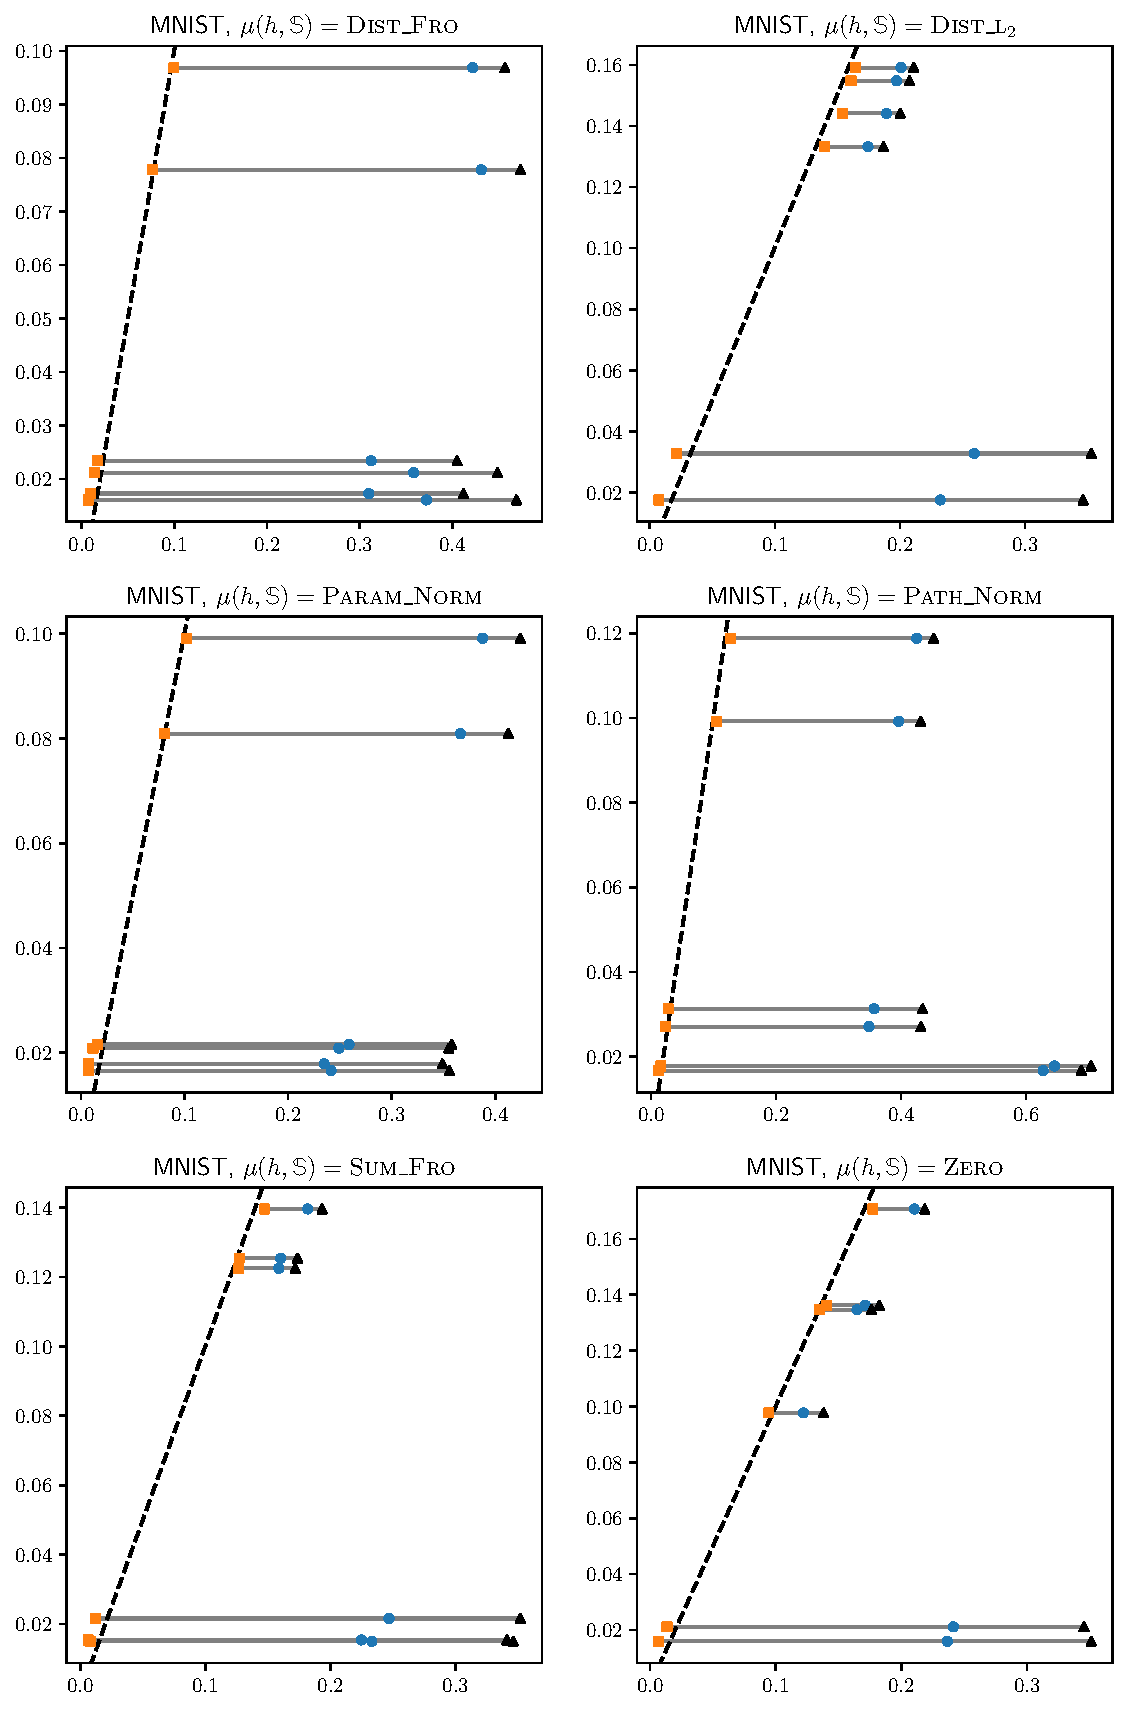
\includegraphics[width=0.77\linewidth]{chapter_7/figures/gap_mnist.pdf}
    \caption[Tightness of \Cref{chap:dis-mu:eq:disintegrated-comp-mcallester-risk,chap:dis-mu:eq:disintegrated-comp-seeger-risk} on MNIST]{
    \looseness=-1
    Scatter plot given a parametric function $\comp(\h, \S)$, where each segment represents a neural network $\h_{\wbf}$ learned with a given $\alpha$, width $H$ and depth $L$.
    For each segment, there is a corresponding orange square and a blue circle.
    The orange squares corresponds to the empirical risk $\Risk_{\dS}(\h)$ (x-axis) and test risk $\Risk_{\dT}(\h)$ (y-axis).
    The blue circle \resp the black triangle represents \Cref{chap:dis-mu:eq:disintegrated-comp-seeger-risk} \resp \Cref{chap:dis-mu:eq:disintegrated-comp-mcallester-risk} in the x-axis and the test risk $\Risk_{\dT}(\h)$ in the y-axis.
    The dashed line is the identity function.
    }
    \label{chap:dis-mu:fig:gap-mnist}
\end{figure}

\begin{figure}
    \centering
    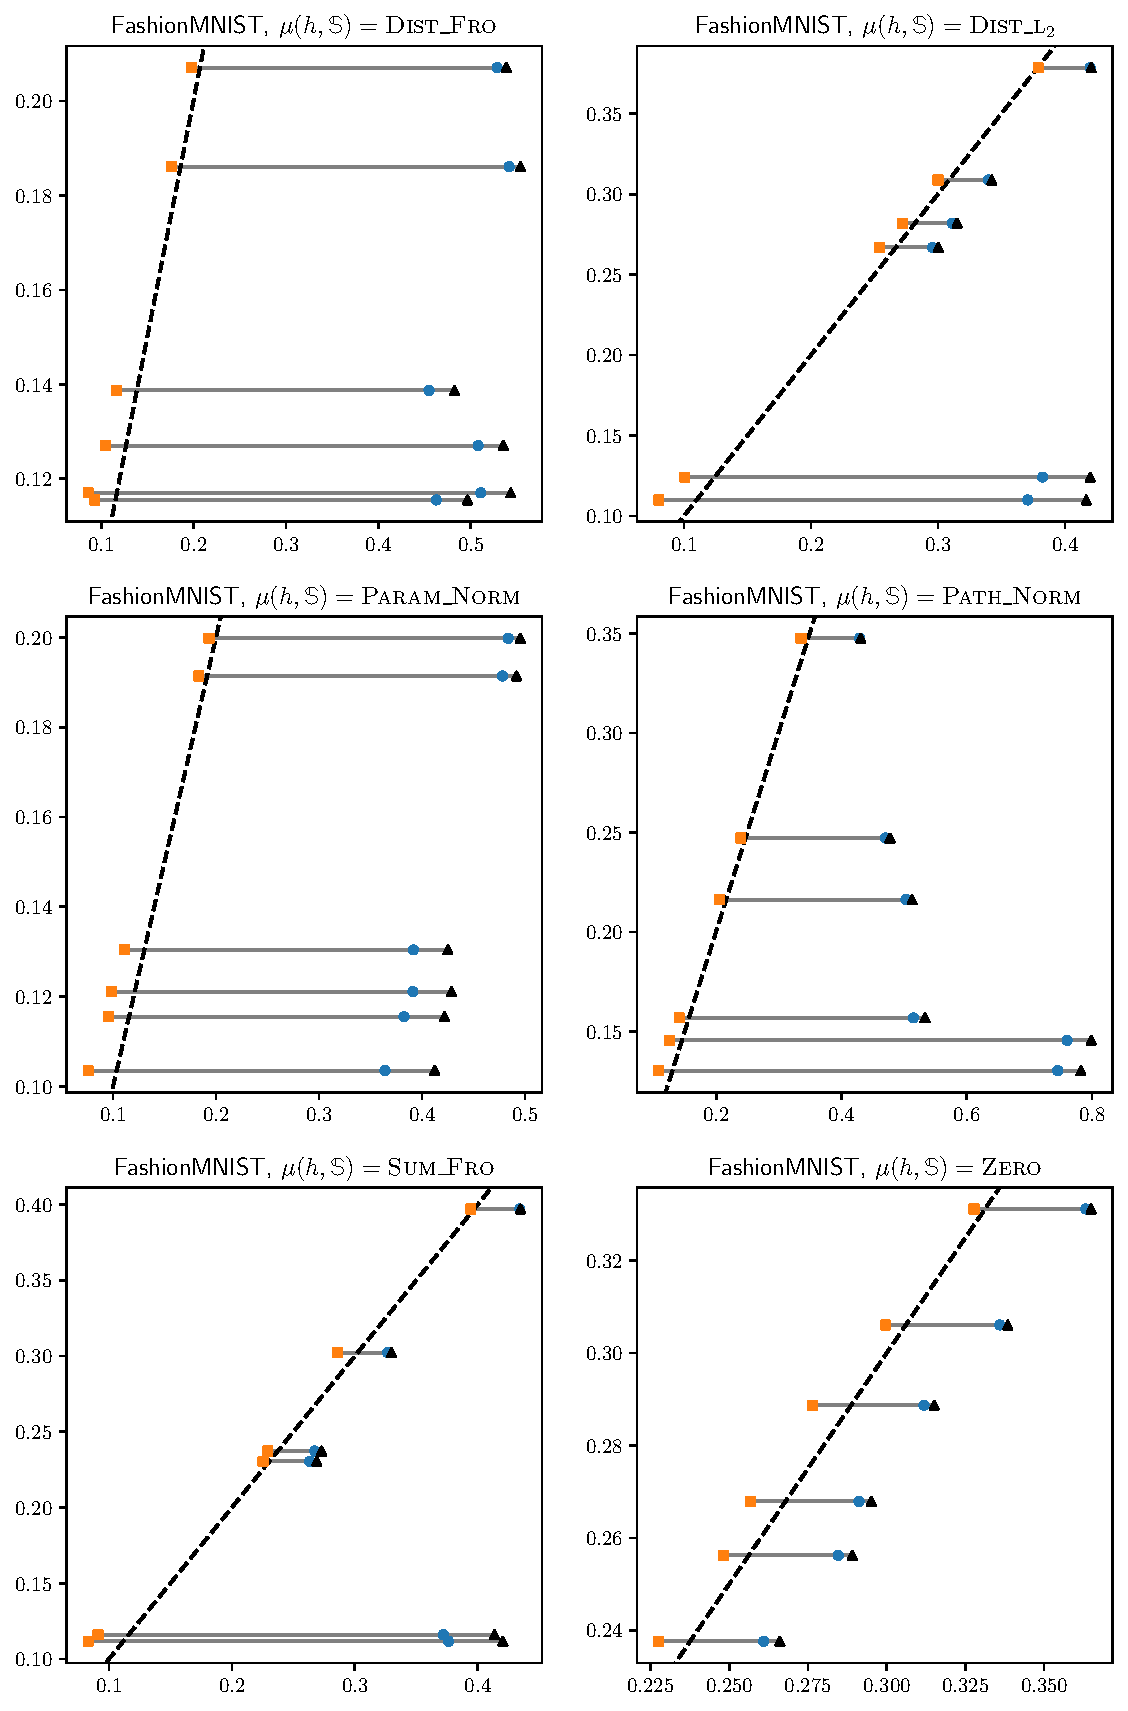
\includegraphics[width=0.77\linewidth]{chapter_7/figures/gap_fashion.pdf}
    \caption[Tightness of \Cref{chap:dis-mu:eq:disintegrated-comp-mcallester-risk,chap:dis-mu:eq:disintegrated-comp-seeger-risk} on FashionMNIST]{
    \looseness=-1
    Scatter plot given a parametric function $\comp(\h, \S)$, where each segment represents a neural network $\h_{\wbf}$ learned with a given $\alpha$, width $H$ and depth $L$.
    For each segment, there is a corresponding orange square and a blue circle.
    The orange squares corresponds to the empirical risk $\Risk_{\dS}(\h)$ (x-axis) and test risk $\Risk_{\dT}(\h)$ (y-axis).
    The blue circle \resp the black triangle represents \Cref{chap:dis-mu:eq:disintegrated-comp-seeger-risk} \resp \Cref{chap:dis-mu:eq:disintegrated-comp-mcallester-risk} in the x-axis and the test risk $\Risk_{\dT}(\h)$ in the y-axis.
    The dashed line is the identity function.
    }
    \label{chap:dis-mu:fig:gap-fashion}
\end{figure}

\begin{figure}
    \centering
    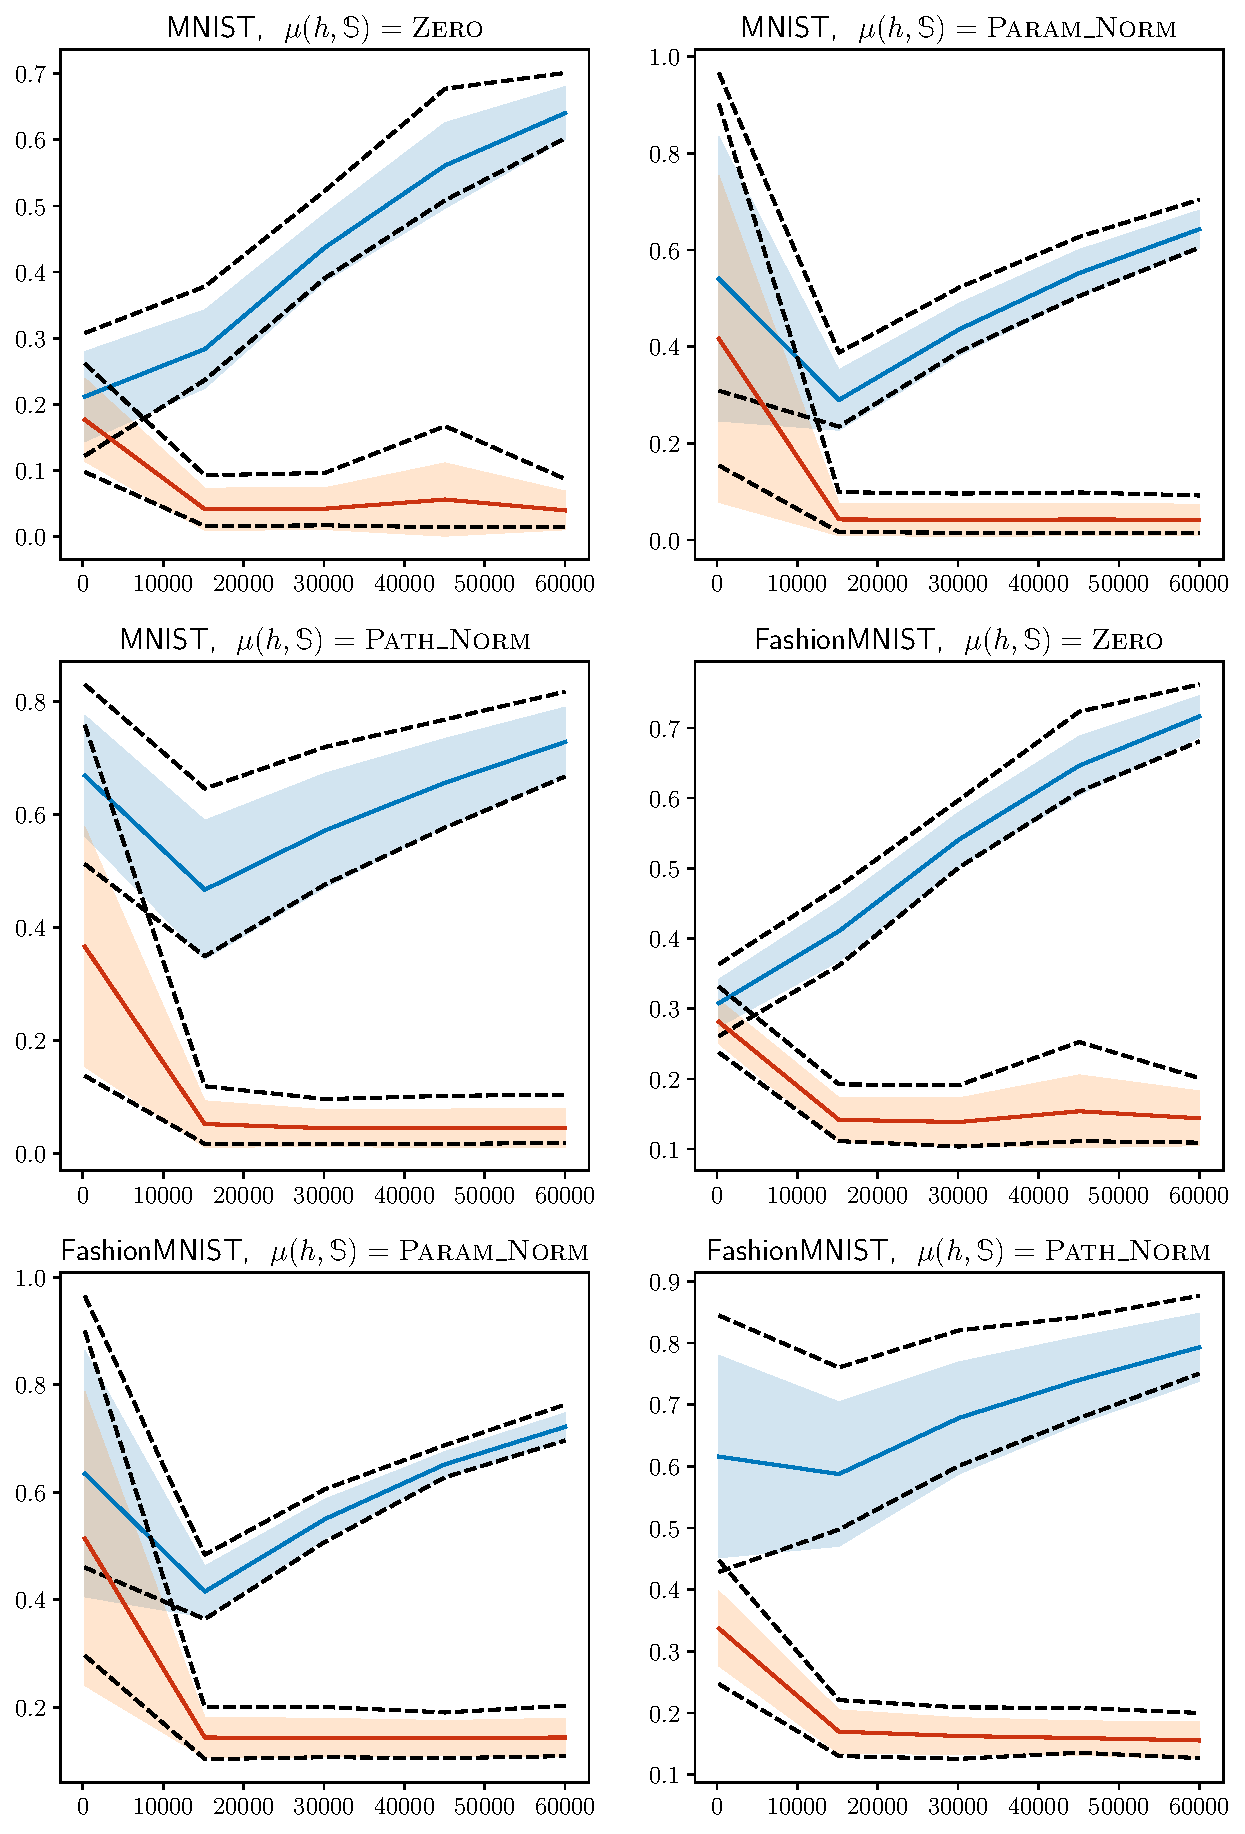
\includegraphics[width=0.82\linewidth]{chapter_7/figures/influence_alpha_summary.pdf}
    \caption[Influence of the Parameter $\alpha$]{
    \looseness=-1
    Influence of the parameter $\alpha$ (in the x-axis) for three parametric functions: $\zero$, $\paramnorm$, and $\pathnorm$ for MNIST and FashionMNIST.
    The bound values are represented in blue and the test risk in red. 
    The two (solid) lines are the mean values computed on the depths and widths; the shadows are the standard deviation.
    The dashed lines are the minimum and the maximum values.
    }
    \label{chap:dis-mu:fig:influence-alpha}
\end{figure}

\begin{figure}
    \centering
    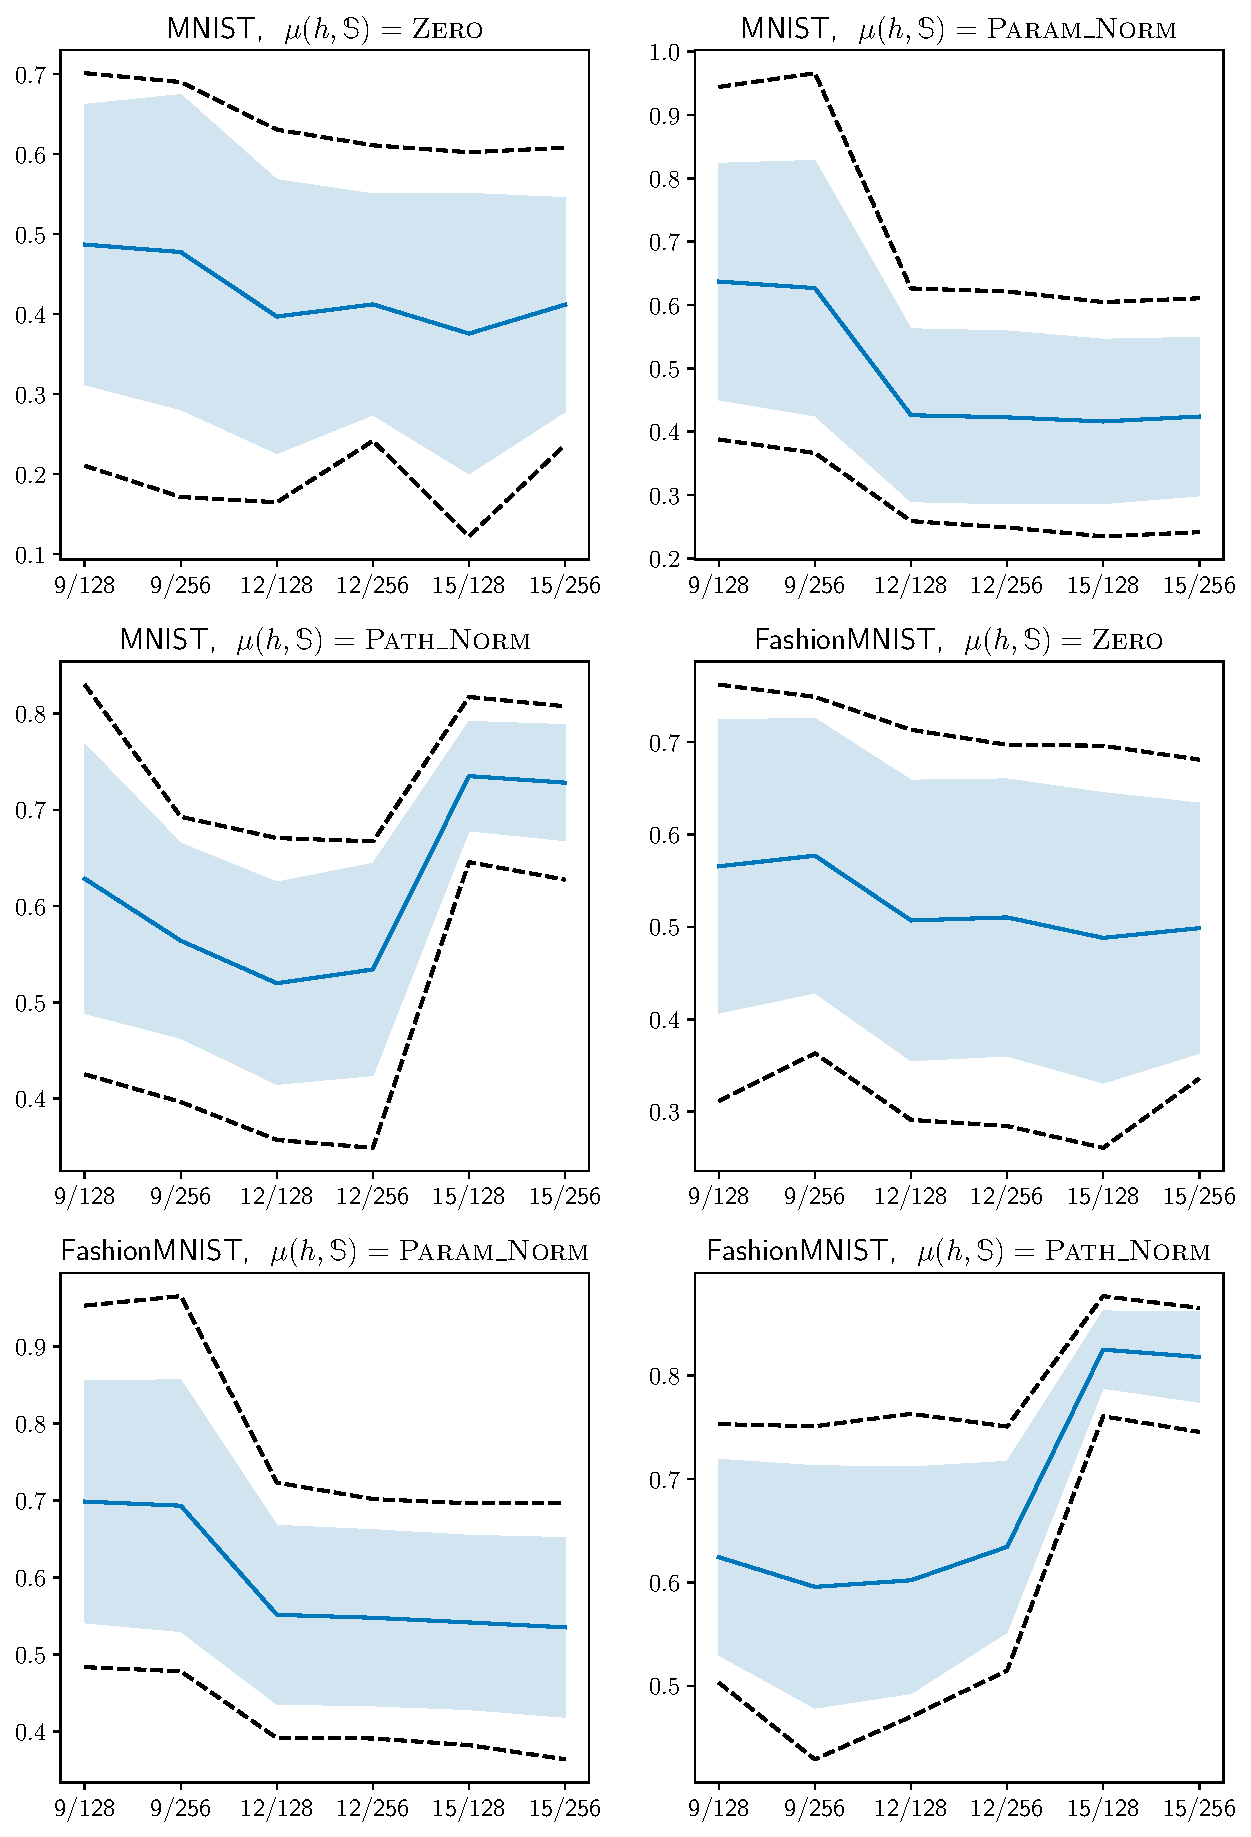
\includegraphics[width=0.82\linewidth]{chapter_7/figures/influence_depth_summary.pdf}
    \caption[Influence of the Depth/Width]{
    \looseness=-1
    Influence of the depth and the width (in the x-axis as ``depth/width'') for three parametric functions: $\zero$, $\paramnorm$, and $\pathnorm$ for MNIST and FashionMNIST.
    The (solid) lines are the mean values computed on the different values of $\alpha$; the shadows are the standard deviation. 
    The dashed lines are the minimum and the maximum values.
    }
    \label{chap:dis-mu:fig:influence-depth}
\end{figure}

For each parametric function $\comp()$, we report in \Cref{chap:dis-mu:fig:gap-mnist,chap:dis-mu:fig:gap-fashion}, the test risks $\Risk_{\dT}(\h)$ and the values of the tightest bound (\wrt $\alpha$) associated to \Cref{chap:dis-mu:eq:disintegrated-comp-seeger-risk,chap:dis-mu:eq:disintegrated-comp-mcallester-risk} for different parameters (depth $L$, width $H$).
First of all, we can remark that certain empirical risks are high.
This is due to the sampling of the hypothesis $\h$ from the distribution $\AQ$: the hypothesis does not necessarily minimizes the objective function $\h \mapsto \Risk_{\dS}(\h){+}\frac{1}{\alpha}\comp(\h, \S)$.
We can nevertheless observe that the bounds' values are higher when the empirical risk $\Risk_{\dT}(\h)$ is low.
This can be explained by the fact that $\LB\alpha\Risk_{\dS}(\h{'})  + \comp(\h'\!,\S)\RB - \LB\alpha\Risk_{\dS}(\h)+\comp(\h,\S)\RB$ is large in this case.
When the empirical risks are a bit higher, the bounds become tighter for certain parametric function such as $\distltwo$, $\sumfro$. 
This confirms that there is an interest to use a parametric function that captures information on the model during the training phase.

\subsubsection{Influence of the Parameter $\alpha$}
\label{chap:dis-mu:sec:influence-alpha}

We analyze the influence of the parameter $\alpha$ in \Cref{chap:dis-mu:eq:disintegrated-comp-seeger-risk}.
To do so, we plot an overview of the evolution for the bounds and the test risks $\Risk_{\dT}(\h)$; the details are reported in \Cref{ap:dis-mu}. 
For each parameter $\alpha$, we plot in \Cref{chap:dis-mu:fig:influence-alpha} the mean, the standard deviation, the minimum and the maximum for the different parameters (depth and width).
In general, the bound increases when the $\alpha$ tends to $\m$ but the test risks $\Risk_{\dT}(\h)$ are less prone to variations.
Indeed, the higher the parameter $\alpha$, the more concentrated around the minimizers the hypothesis will be sampled.
On the contrary, for a small $\alpha$ (\eg, $\alpha=\sqrt{\m}$), the Gibbs distribution defined in \Cref{chap:dis-mu:eq:gibbs-distribution} is less concentrated making the test risks potentially high with a tighter generalization bound.

\subsubsection{Influence of the Depth/Width}
\label{chap:dis-mu:sec:influence-depth}

In \Cref{chap:dis-mu:fig:influence-depth}, we show an overview of the evolution of \Cref{chap:dis-mu:eq:disintegrated-comp-seeger-risk} with respect to the depth and the width.
More precisely, we report the mean, the standard deviation, the minimum and the maximum values for three parametric functions ($\zero$, $\paramnorm$, and $\pathnorm$).

Interestingly, the evolution of the bounds highly depends on the chosen parametric function $\comp()$. 
For instance, the bound increases with $\pathnorm$ when the depth and the width increase.
This is in contrast with $\paramnorm$ that decreases when the number of parameters increases.
This shows the interest of our framework: considering a user-specified complexity measure $\PhiComp()$ can help to understand the generalization of over-parameterized models (that are sampled from $\AQ$).

\section{Comparison with the Generalization Bounds of the Literature}
\label{chap:dis-mu:sec:comparison}

In this section, we theoretically compare generalization bounds with arbitrary complexity measures compared to literature's bounds. 
We prove that our bound generalizes the uniform-convergence and the algorithmic-dependent bounds.
Additionally, we show that the algorithmic-dependent bounds can be tighter than uniform-convergence bounds.
To do so, we propose in \Cref{chap:dis-mu:proposition:disintegrated,chap:dis-mu:proposition:uc,chap:dis-mu:proposition:algorithmic} a reinterpretation of the high probability bounds in terms of sets.
Additionally, we prove in \Cref{chap:dis-mu:corollary:dis-uc,chap:dis-mu:corollary:dis-algo} two special cases of our bound in \Cref{chap:dis-mu:theorem:disintegrated-comp} that generalizes the two types of bounds.

\subsection{Bounds with Arbitrary Complexity Measures}

In order to compare our framework with the uniform-convergence and the algorithmic-dependent bounds, we translate \Cref{chap:dis-mu:def:comp-bound} into the following set-theoretic result.

\begin{restatable}[Set-theoretic view of \Cref{chap:dis-mu:def:comp-bound}]{proposition}{propositiondisintegrated}\label{chap:dis-mu:proposition:disintegrated}
Let $\phi: [0,1]^2{\to}\Rbb$ be a generalization gap and assume that there exists a function $\PhiComp: \H{\times}(\X{\times}\Y)^\m{\times}(0,1]\to\Rbb$ fulfilling \Cref{chap:dis-mu:def:comp-bound}.
Under these conditions, with $\setD {=} \Big\{ (\h, \S)\!\in\! \H{\times}(\X{\times}\Y)^\m :  \phi(\Risk_{\D}(\h), \Risk_{\dS}(\h))\!\le\!\PhiComp(\h, \S, \delta) \Big\}$, and  $\PP_{\S\sim\D^\m, h\sim\AQ}\LB (\h, \S)\in\setD \RB\ge  1{-}\delta$, we have
\begin{align*}
    \text{\Cref{chap:dis-mu:eq:comp-bound}} \iff\ &\forall (\h, \S)\in \setD,\  \phi(\Risk_{\D}(\h), \Risk_{\dS}(\h)) \le \PhiComp(\h, \S, \delta)\\
 \iff\ &  {\textstyle\sup_{(\h, \S)\in \setD}} \Big\{\phi(\Risk_{\D}(\h), \Risk_{\dS}(\h)) - \PhiComp(\h, \S, \delta) \Big\} \le 0.
\end{align*}
\end{restatable}
\begin{noaddcontents}\begin{proof}
Deferred to~\Cref{ap:dis-mu:sec:proof-prop-disintegrated}.
\end{proof}\end{noaddcontents}
For a given confidence $\delta$, with probability at least $1{-}\delta$,
the bound is then valid for all $(\h, \S)$ belonging to a (reduced) set $\setD \!\subseteq\! \H{\times}(\X{\times}\Y)^\m$.
In other words, the bound always holds for a given hypothesis and learning sample $(\h, \S)\!\in\!\setD$, and its value depends on these $\h$ and $\S$.  
The generality of our framework can thus generalize both uniform convergence and algorithmic dependent bounds as we see in the rest of this section. 

\subsection{Uniform Convergence Bounds}

\looseness=-1
Uniform-convergence-based bounds were the first type of generalization bounds to be introduced, notably in \citet{VapnikChervonenkis1971} using the VC-dimension as complexity.
Other bounds were later developed based on the Gaussian/Rademacher complexity~\citep{BartlettMendelson2002} instead.
We recall the definition of this type of bounds encountered in \Cref{chap:intro}.

\definitionUC*

Remember that this definition encompasses different complexity measures, such as $\PhiUC(\delta){=}\rad(\H) {+} \sqrt{\tfrac{1}{2\m}\ln\frac{1}{\delta}}$ in \Cref{chap:intro:theorem:rademacher}, or $\PhiUC(\delta){=}\sqrt{\frac{1}{m}2\vc(\H)\ln\frac{em}{\vc(\H)}}{+}\sqrt{\tfrac{1}{2\m}\ln\frac{1}{\delta}}$ described in \Cref{chap:intro:theorem:vc-dim}.
For ease of comparison, we refine and reinterpret this type of bounds in a set-theoretic manner as follows.
This result has been originally remarked by \citet{NagarajanKolter2019} (but not proved).

\begin{restatable}[Set-theoretic View of Uniform Convergence Bounds]{proposition}{propositionuc}\label{chap:dis-mu:proposition:uc}
Let $\phi: [0,1]^2{\to}\Rbb$ be a generalization gap and assume that there exists a function $\PhiUC: (0,1]\to\Rbb$ fulfilling \Cref{chap:intro:def:uc}.
Under these conditions, with $\displaystyle\setUC = \big\{ \S\in (\X{\times}\Y)^\m \!:\! \forall \h\in\H,\, \phi(\Risk_{\D}(\h), \Risk_{\dS}(\h)) \le \PhiUC(\delta) \big\}$, and $\PP_{\S\sim\D^\m}\LB \S{\in}\setUC \RB{\ge}  1{-}\delta$, we have
\begin{align*}
    \text{\Cref{chap:intro:eq:uc}} &\iff \forall \S \in \setUC,\   \forall h\!\in\! \H,\, \phi(\Risk_{\D}(\h), \Risk_{\dS}(\h)) \le \PhiUC(\delta)\\
    &\iff \sup_{\S\in\setUC}\sup_{h\in\H}\big\{\phi(\Risk_{\D}(\h), \Risk_{\dS}(\h))\big\}\! \le\! \PhiUC(\delta).
\end{align*}
\end{restatable}
\begin{noaddcontents}\begin{proof}
Deferred to~\Cref{ap:dis-mu:sec:proof-prop-uc}.
\end{proof}\end{noaddcontents}

\Cref{chap:dis-mu:proposition:uc} is, in fact, a reinterpretation of PAC generalization bounds by identifying the subset $\setUC {\subseteq} (\X{\times}\Y)^\m$ for which the upper bound $\PhiUC(\delta)$ is valid.
This highlights their worst-case nature:
given a confidence $\delta$, the generalization gap $\phi(\Risk_{\D}(\h), \Risk_{\dS}(\h))$ is upper-bounded by a complexity measure $\PhiUC(\delta)$ for all $(\h,\S)\!\in\!\H{\times}\setUC$.
To get a bound holding with probability at least $1{-}\delta$, 
since the complexity $\PhiUC(\delta)$ does not depend on $\h$ or $\S$, the complexity has to upper-bound the worst hypothesis $\h\!\in\!\H$ and the worst learning sample $\S\!\in\!\setUC$. 
As a consequence, $\PhiUC(\delta)$ is lower-bounded by $\sup_{\S\in\setUC}\sup_{h\in\H}\phi(\Risk_{\D}(\h), \Risk_{\dS}(\h))$.
As we have seen in \Cref{chap:dis-mu:proposition:disintegrated}, our bound is more permissive than the uniform convergence bounds since the upper bound can depend on the learning sample $\S$ and the hypothesis $\h$.
Hence, this dependence on $\S$ and $\h$ allows us to retrieve the uniform convergence bounds with our framework.
Indeed, from \Cref{chap:dis-mu:theorem:disintegrated-comp}, we can obtain the following generalization bound.

\begin{restatable}[Uniform Convergence Bound from \Cref{chap:dis-mu:theorem:disintegrated-comp}]{corollary}{corollarydisuc} \label{chap:dis-mu:corollary:dis-uc}
Let $\phi\!:\! [0,1]^2{\to}\Rbb$ be the generalization gap and assume that there exists a function $\PhiUC: (0,1]\to\Rbb$ fulfilling \Cref{chap:intro:def:uc} such that $\PhiUC(\delta) \ge \ln\!\LB \frac{4}{\delta^2} \EE_{\S'\!{\sim}\D^\m}\EE_{\h'\!{\sim}\P} \exp\LP\phi(\Risk_{\D}(\h{'}),\Risk_{\dS'}(\h'))\RP\RB$.
For any $\D$ on $\X\times\Y$, for any hypothesis set $\H$, for any $\delta\in(0, 1]$, we have
\begin{align*}
    \PP_{\S\sim\D^\m, \h\sim\AQ}\!\Bigg[ \phi(\Risk_{\D}(\h), \Risk_{\dS}(\h)) \le \PhiUC(\delta) \Bigg] \ge 1-\delta.
\end{align*}
\end{restatable}
\begin{noaddcontents}\begin{proof}
Deferred to~\Cref{ap:dis-mu:sec:proof-cor-dis-uc}.
\end{proof}\end{noaddcontents}

Note that, to prove \Cref{chap:dis-mu:corollary:dis-uc}, we require an additional assumption: a lower-bound on $\PhiUC(\delta)$.
When the generalization gap is $\phi(\Risk_{\D}(\h), \Risk_{\dS}(\h)){=}2m[\Risk_{\D}(\h){-}\Risk_{\dS}(\h)]^2$ or $\phi(\Risk_{\D}(\h), \Risk_{\dS}(\h)){=}\kl[\Risk_{\dS}(\h)\|\Risk_{\D}(\h)]$, the lower bound is $\ln\frac{8\sqrt{\m}}{\delta^2}$ (see \Cref{chap:dis-mu:corollary:disintegrated-comp}) which is low enough to be a worst-case upper-bound.
To sum up, our framework is general enough to retrieve classical uniform convergence bounds (under the mild assumption) such that the ones based on the Rademacher complexity (\Cref{chap:intro:def:rademacher}) or the VC-Dimension (\Cref{chap:intro:def:vc-dim}).
In practice, the sampling involved in the bound of \Cref{chap:dis-mu:corollary:dis-uc} is not necessary: the bound holds for all hypothesis $\h\in\H$ with high probability.
More precisely, for $\PhiUC(\h,\S,\delta)=\PhiUC(\delta)$, the set $\setUC$ in \Cref{chap:dis-mu:proposition:uc} can be seen as a subset of $\setD$ since
\begin{align*}
    \Big\{ \S\in(\X{\times}\Y)^\m \;\Big|\; \forall \h\in\H,\ (\S,\h)\in\setD \Big\} = \setUC.
\end{align*}
Hence, for a well-behaved learning sample $\S$, \ie, for $\S\in\setUC$, we have that
\begin{align*}
    \EE_{\h\in\AQ}\indic\Big[ \phi(\Risk_{\D}(\h), \Risk_{\dS}(\h)) \le \PhiUC(\delta) \Big] &= \indic\LB \sup_{\h\in\H}\phi(\Risk_{\D}(\h), \Risk_{\dS}(\h)) \le \PhiUC(\delta) \RB\\
    &= 1,
\end{align*}
which gives a valid bound for all $\h\in\H$ without sampling.
This generality of this framework does not apply uniquely to these type of bounds. 
We can obtain a result similar for the algorithmic-dependent bounds that can be tighter than the uniform-convergence-based bounds. 

\subsection{Algorithmic-Dependent Bounds}

\looseness=-1
The upper bound $\PhiUC(\delta)$ can generally be improved by considering algorithmic-dependent bounds~\citep{BousquetElisseeff2002, XuMannor2012}.
In this case, only the output $\h_{\S}$ of a learning algorithm given $\S$ is studied: we only bound the generalization gap $\phi(\Risk_{\D}(\h_{\S}), \Risk_{\dS}(\h_{\S}))$ specific to $\h_{\S}$ (here,  $\H{=}\{\h_{\S}\}_{\S\in(\X{\times}\Y)^\m}$).
The definition of such bounds encountered in \Cref{chap:intro} is recalled in the following.

\definitionALGODEP*

Similarly to the uniform convergence bounds, these bounds can be reformulated through a similar set-theoretic lens stated in the following proposition.

\begin{restatable}[Set-theoretic View of Algorithmic Dependent Bounds]{proposition}{propositionalgodep}\label{chap:dis-mu:proposition:algorithmic}
\looseness=-1
Let $\phi: [0,1]^2{\to}\Rbb$ be a generalization gap and assume that there exists a function $\PhiA: (0,1]\to\Rbb$ fulfilling \Cref{chap:intro:def:algo}.
Under these conditions, with $\setA = \big\{ \S\in (\X{\times}\Y)^\m \!:\! \phi(\Risk_{\D}(\h_{\S}), \Risk_{\dS}(\h_{\S}))\le\PhiA(\delta) \big\}$ and $\PP_{\S{\sim}\D^\m}\!\LB \S\in\setA \RB\ge  1{-}\delta$, we have
\begin{align*}
    \text{\Cref{chap:intro:eq:algo}}\ &\iff \forall\S\in\setA,  \phi(\Risk_{\D}(\h_{\S}), \Risk_{\dS}(\h_{\S})) \le \PhiA(\delta)\\
    &\iff {\textstyle \sup_{\S\in\setA}} \phi(\Risk_{\D}(\h_{\S}), \Risk_{\dS}(\h_{\S})) \le \PhiA(\delta). 
\end{align*}
\end{restatable}
\begin{noaddcontents}\begin{proof}
Deferred to~\Cref{ap:dis-mu:sec:proof-prop-algo}.
\end{proof}\end{noaddcontents}
Since the upper bound $\PhiA(\delta)$ is at least $\sup_{\S\in\setA}\phi(\Risk_{\D}(\h_{\S}), \Risk_{\dS}(\h_{\S}))$, this result has the potential to lead to tighter guarantees than the uniform convergence ones.
For example, when $\H {=} \LC \h_{\S}\RC_{\S\in(\X{\times}\Y)^\m}$ is an algorithmic-dependent hypothesis set and $\setA\!\subseteq\!\setUC$.
The complexity measure $\PhiA(\delta)$ can potentially be smaller than $\PhiUC(\delta)$ since we have the inequality 
\begin{align*}
\sup_{\S\in\setA}\phi(\Risk_{\D}(\h_{\S}), \Risk_{\dS}(\h_{\S})) &\le \sup_{\S\in\setUC}\phi(\Risk_{\D}(\h_{\S}), \Risk_{\dS}(\h_{\S}))\\
&\le \sup_{\S\in\setUC}\sup_{\h\in\H}\phi(\Risk_{\D}(\h), \Risk_{\dS}(\h))\\
&\le \PhiUC(\delta).
\end{align*}
Even though these type of bounds can be tighter, it is still not as permissive as our framework.
Indeed, the upper bound $\PhiA(\delta)$ is a constant \wrt the hypothesis and the learning sample (like the uniform convergence bounds).
Hence, since our bound can depend on the learning sample $\S$ and the hypthesis $\h$, we retrieve the algorithmic-dependent bounds illustrating the generality of our framework (similarly to \Cref{chap:dis-mu:corollary:dis-uc}).
The result is in the following corollary.

\begin{restatable}[Algorithmic-dependent Bound from \Cref{chap:dis-mu:theorem:disintegrated-comp}]{corollary}{corollarydisalgo} \label{chap:dis-mu:corollary:dis-algo}
Let $\phi\!:\! [0,1]^2{\to}\Rbb$ be the generalization gap and assume that there exists a function $\PhiA: (0,1]\to\Rbb$ fulfilling \Cref{chap:intro:def:algo} such that $\PhiA(\delta) \ge \ln\!\LB \frac{4}{\delta^2} \EE_{\S'\!{\sim}\D^\m}\EE_{\h'\!{\sim}\P} \exp\LP\phi(\Risk_{\D}(\h{'}),\Risk_{\dS'}(\h'))\RP\RB$.
For any $\D$ on $\X\times\Y$, for any hypothesis set $\H$, for any $\delta\in(0, 1]$, we have
\begin{align*}
    \PP_{\S\sim\D^\m, \h\sim\AQ}\!\Bigg[ \phi(\Risk_{\D}(\h), \Risk_{\dS}(\h)) \le \PhiA(\delta) \Bigg] \ge 1-\delta.
\end{align*}
\end{restatable}
\begin{noaddcontents}\begin{proof}
Deferred to~\Cref{ap:dis-mu:sec:proof-corollary-algo}.
\end{proof}\end{noaddcontents}

Compared to the bounds of \Cref{chap:intro:def:algo}, \Cref{chap:dis-mu:corollary:dis-algo} still involves the expectation over the hypotheses. 
Hopefully, the bound holds with high probability for the data-dependent hypothesis $\h_{\S}$ (see \Cref{chap:dis-mu:proposition:algorithmic}).
Hence, when using \Cref{chap:dis-mu:corollary:dis-algo}'s bound the sampling is not necessary since we can consider the bound only for the hypothesis of interest, \ie, $\h_{\S}$ for all $\S\in\setA$ which holds with high probability.
In other words, when $\PhiComp(\h,\S,\delta) = \PhiA(\delta)$, the set $\setA$ in \Cref{chap:dis-mu:proposition:algorithmic} can be seen as a subset of $\setD$ since
\begin{align*}
    \Big\{ \S\in(\X{\times}\Y)^\m \;\Big|\; (\S,\h_{\S})\in\setD \Big\} = \setA.
\end{align*}

In summary, the framework proposed in this chapter is powerful enough to cover uniform-convergence-based bound and algorithm-dependent bounds with the integration of a complexity measure. 
To the best of our knowledge, this has not been identified before and we think this is something novel.

\section{Conclusion and Summary}
\label{chap:dis-mu:sec:conclu}

In this chapter, we provide a novel generalization bound that involves arbitrary complexity measures, unlike classical learning theory frameworks (for which the complexity is imposed by the framework itself).
These measures incorporate a data and model dependent function, that allow us to generalize the previous framework introduced in the literature (see \Cref{chap:intro:sec:bound}).
Importantly, to the best of our knowledge, our framework provides for the first time theoretical guarantees for the many arbitrary complexity measures used in practice in machine learning, \eg,  for regularization purposes.\\

The limitation of this work is clearly that the hypothesis is obtained from a distribution difficult to use, namely the Gibbs distribution.
Indeed, one sampling from the Gibbs distribution is performed by an algorithm such as \Cref{chap:dis-mu:algo:sto-mala}.
Hopefully, the generality of this framework allows to avoid the sampling if we consider uniform-convergence-type bounds as in \Cref{chap:dis-mu:corollary:dis-uc}.
We can easily imagine continuing in this research direction.
For instance, we can try to get rid of the supremum \wrt to the hypothesis set $\H$ in the Rademacher complexity (\Cref{chap:intro:def:rademacher}) since it it hard to compute.

We hope that our results foster research in the topic and the development of new complexity measures for specific neural network architectures and for specific learning tasks.
Indeed, we believe that this work paves the way to new research directions that tries to bridge the statistical learning theory and the practice.
Indeed, finding a good complexity measures becomes a practical matter since any complexity measure can be integrated in our framework.\\

In general, this thesis explores the disintegrated bounds in order to explain better the generalization of over-parameterized models that is largely misunderstood. 
We believe that this type of bounds is not the only promising type of bounds that can explain the generalization phenomenon.
In \Cref{part:conclusion}, we give an idea of research direction to explore other type of generalization bounds.